\documentclass[11pt,twocolumn]{article}

\usepackage[utf8]{inputenc}
\usepackage[T1]{fontenc}
\usepackage[a4paper,margin=1.75cm,columnsep=0.7cm]{geometry}
\usepackage{booktabs}
\usepackage{array}
\usepackage{hyperref}
\usepackage{xcolor}
\usepackage{graphicx}
\usepackage{tikz}
\usetikzlibrary{arrows.meta,positioning,shapes.geometric}

\hypersetup{
  colorlinks=true,
  linkcolor=black,
  urlcolor=blue
}

\setlength{\parindent}{0pt}
\setlength{\parskip}{3pt}

\tikzset{
  entity/.style={
    draw,
    rounded corners=1mm,
    fill=blue!5,
    align=left,
    font=\scriptsize,
    text width=3.15cm,
    minimum height=1.15cm,
    inner sep=3pt
  },
  fact/.style={
    draw,
    rounded corners=1mm,
    fill=orange!10,
    align=left,
    font=\scriptsize,
    text width=4.2cm,
    minimum height=1.45cm,
    inner sep=3pt
  },
  rel/.style={-{Latex[length=2mm]}, line width=0.45pt}
}

\title{\vspace{-1.1cm}\textbf{Election Analytics Platform for Portugal}\\
\large Advanced Topics in Databases Practical Assignment}
\author{
Rui Coelho, up202106772 \and
Ricardo Ribeiro, up202104806
}
\date{June 2026}

\begin{document}
\maketitle

\begin{abstract}
This project implements a database-centred analytics platform for the Portuguese 2021 local elections. The system loads official CNE election spreadsheets into PostgreSQL/PostGIS through a rerunnable ETL pipeline, normalizes the data into an operational schema, populates a dimensional warehouse, and exposes the results through a thin Flask application using explicit SQL through \texttt{psycopg2}. The database includes functions, PL/pgSQL procedures, triggers, materialized views, analytical SQL, D'Hondt mandate allocation, and CAOP administrative geometries for district and municipality-level map visualization.
\end{abstract}

\section{Scope and Data Sources}

The project focuses on the 2021 Portuguese local elections (\emph{Eleições Autárquicas 2021}). This scope was chosen because the assignment recommends it as a baseline and because the CNE provides an official spreadsheet package with detailed results for municipal councils, municipal assemblies, and parish assemblies.

The main official election data source is the CNE package \texttt{2021al\_mapa\_oficial}, containing:

\begin{itemize}
  \item \texttt{mapa\_1\_resultados.xlsx}: registered voters, voters, blank votes, null votes, and votes per candidacy;
  \item \texttt{mapa\_anexo.xlsx}: local resolution of labels such as \texttt{[A]}, \texttt{[B]}, and citizen-group candidacies;
  \item \texttt{mapa\_2\_perc\_mandatos.xlsx}: official vote percentages and mandates;
  \item \texttt{mapa\_3\_eleitos.xlsx}: elected members by territory, organ, and list.
\end{itemize}

For administrative boundaries, the project uses DGT CAOP GeoPackage files. The available files are CAOP 2025 rather than CAOP 2021. This is a limitation, but it is a compatible official DGT administrative-boundary dataset and is explicitly documented. The election facts remain from 2021; the geometries are used for visualization and spatial storage.

\section{Architecture}

The system is organized around the database. Python is used for ETL and as a thin web layer, but the analytical logic remains explicit in SQL and PL/pgSQL.

\begin{itemize}
  \item \texttt{staging}: raw CNE rows transformed from Excel into relational staging tables;
  \item \texttt{election}: normalized operational schema;
  \item \texttt{dw}: dimensional warehouse for analytical queries;
  \item \texttt{app}: Flask frontend using \texttt{psycopg2};
  \item \texttt{etl}: rerunnable CNE and CAOP loaders.
\end{itemize}

The loading sequence is: parse CNE Excel files, copy rows into staging, call \texttt{election.load\_from\_staging()}, call \texttt{dw.refresh\_from\_operational()}, and refresh materialized views used by the frontend.

The repository structure follows the assignment recommendation. SQL files are placed under \texttt{sql/}; Python ETL scripts under \texttt{etl/}; the Flask frontend under \texttt{app/}; processed data checks under \texttt{data/processed/}; and documentation under \texttt{docs/}. The raw CNE spreadsheet package is kept in \texttt{2021al\_mapa\_oficial/}. CAOP GeoPackages are kept in separate CAOP directories and loaded through the spatial ETL script.

\section{Operational Model}

The operational schema is normalized around elections, organs, territories, candidacies, turnout, votes, seats, and elected members. Parties, coalitions, and citizen groups are unified under \texttt{candidacies}, because the CNE spreadsheets mix fixed party columns with local labels such as \texttt{[A]} and \texttt{[D]}.

\begin{figure*}[t]
\centering
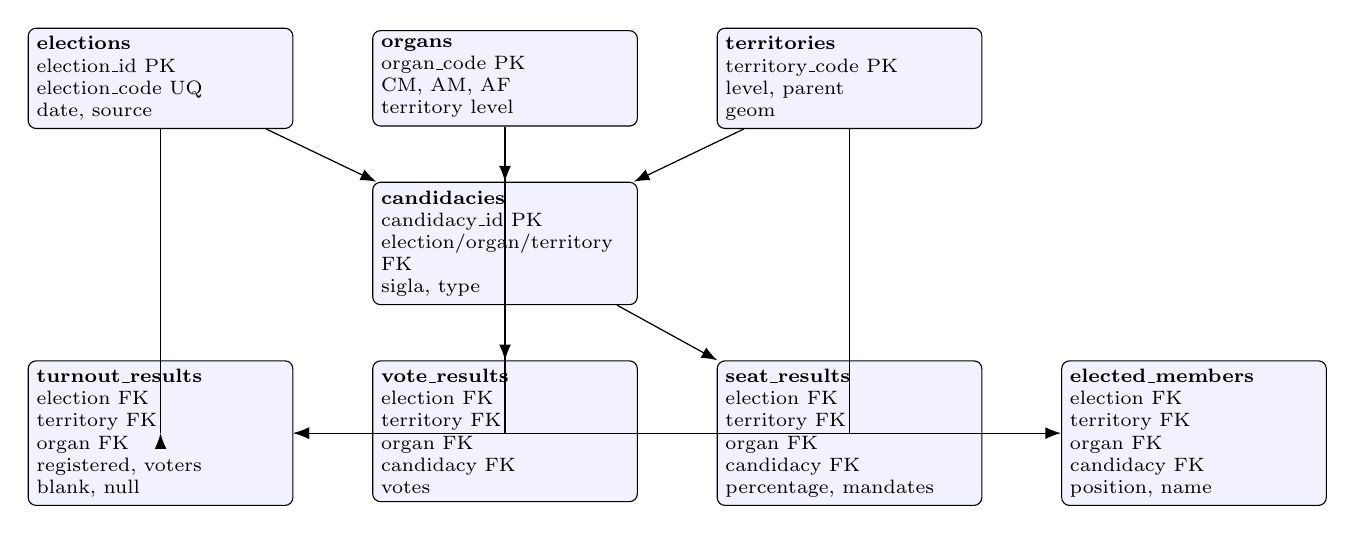
\begin{tikzpicture}[node distance=0.7cm and 1.0cm]
  \node[entity] (elections) {\textbf{elections}\\election\_id PK\\election\_code UQ\\date, source};
  \node[entity, right=of elections] (organs) {\textbf{organs}\\organ\_code PK\\CM, AM, AF\\territory level};
  \node[entity, right=of organs] (territories) {\textbf{territories}\\territory\_code PK\\level, parent\\geom};
  \node[entity, below=of organs] (candidacies) {\textbf{candidacies}\\candidacy\_id PK\\election/organ/territory FK\\sigla, type};

  \node[entity, below left=of candidacies] (turnout) {\textbf{turnout\_results}\\election FK\\territory FK\\organ FK\\registered, voters\\blank, null};
  \node[entity, below=of candidacies] (votes) {\textbf{vote\_results}\\election FK\\territory FK\\organ FK\\candidacy FK\\votes};
  \node[entity, below right=of candidacies] (seats) {\textbf{seat\_results}\\election FK\\territory FK\\organ FK\\candidacy FK\\percentage, mandates};
  \node[entity, right=of seats] (elected) {\textbf{elected\_members}\\election FK\\territory FK\\organ FK\\candidacy FK\\position, name};

  \draw[rel] (elections) -- (candidacies);
  \draw[rel] (organs) -- (candidacies);
  \draw[rel] (territories) -- (candidacies);
  \draw[rel] (elections) |- (turnout);
  \draw[rel] (organs) |- (turnout);
  \draw[rel] (territories) |- (turnout);
  \draw[rel] (candidacies) -- (votes);
  \draw[rel] (candidacies) -- (seats);
  \draw[rel] (candidacies) |- (elected);
\end{tikzpicture}
\caption{Simplified operational ER diagram. Primary entities are elections, organs, territories, and candidacies; result tables reference these dimensions.}
\label{fig:operational-er}
\end{figure*}

Important constraints include unique election codes, unique candidacies per election/organ/territory/source reference, unique vote and seat results per candidacy, and foreign keys from result tables to the core entities. Indexes support territory drill-down, result ranking, spatial lookup through a GiST index, and frontend queries by election, organ, and territory.

The territory hierarchy is represented through \texttt{parent\_code}, \texttt{district\_code}, and \texttt{municipality\_code}. This gives direct access to common drill-down paths without denormalizing result measures. For mainland Portugal, district codes use the pattern \texttt{DD0000}; Madeira is represented as \texttt{300000}; and the Azores as \texttt{400000}. This coding decision reconciles CNE election groupings with CAOP island and regional layers.

The candidacy model is intentionally local to a territory and organ. This is necessary because a label such as \texttt{[A]} has different meanings in different municipalities, and even party coalitions can be local. The schema therefore stores both the source reference and the resolved sigla/name.

\section{ETL Pipeline}

The ETL is implemented in \texttt{etl/load\_cne\_2021.py}. It is rerunnable: staging tables are truncated, source data is reloaded, and the operational and warehouse layers are rebuilt from staging. The project also includes a small XLSX reader in \texttt{etl/xlsx\_reader.py} to avoid depending on Excel-specific tooling for parsing the CNE files.

The ETL performs several cleaning and reconciliation steps:

\begin{itemize}
  \item normalizes territorial codes to six characters;
  \item converts numeric strings into integers or numeric percentages;
  \item resolves local coalition and citizen-group labels using \texttt{mapa\_anexo.xlsx};
  \item stores all candidacies in one structure with a type: party, coalition, or citizen group;
  \item handles region/district code differences for the mainland, Madeira, and the Azores;
  \item loads official percentages and mandates for validation against calculated results.
\end{itemize}

The current parsed counts are shown in Table~\ref{tab:counts}.

\begin{table}[h]
\centering
\caption{CNE ETL row counts.}
\label{tab:counts}
\begin{tabular}{lr}
\toprule
Dataset & Rows\\
\midrule
Result rows & 3719\\
Candidate aliases & 2755\\
Candidate votes & 12277\\
Percentages and mandates & 12277\\
Elected members & 35491\\
\bottomrule
\end{tabular}
\end{table}

The ETL uses PostgreSQL \texttt{COPY} through \texttt{psycopg2} for staging inserts, which is faster and simpler than row-by-row inserts. The transformation from staging to operational tables is then handled inside the database by PL/pgSQL. This separation keeps Python responsible for file parsing and PostgreSQL responsible for relational reconciliation, constraints, and analytical preparation.

The CAOP ETL is implemented separately in \texttt{etl/load\_caop.py}. It reads GeoPackage layers whose names contain \texttt{municipios}, \texttt{distritos}, and \texttt{freguesias}, reprojects all geometries to EPSG:3763, normalizes territorial codes, dissolves duplicate administrative units where necessary, and updates the existing territory rows. This avoids inserting geometries that are not linked to election results.

\section{Data Warehouse}

The warehouse follows a star-schema style. The central fact table is \texttt{dw.fact\_election\_results}, with dimensions for election, organ, territory, and candidacy. This supports comparisons across territories, candidacies, and election organs while keeping analytical queries simpler than the fully normalized operational schema.

\begin{figure*}[t]
\centering
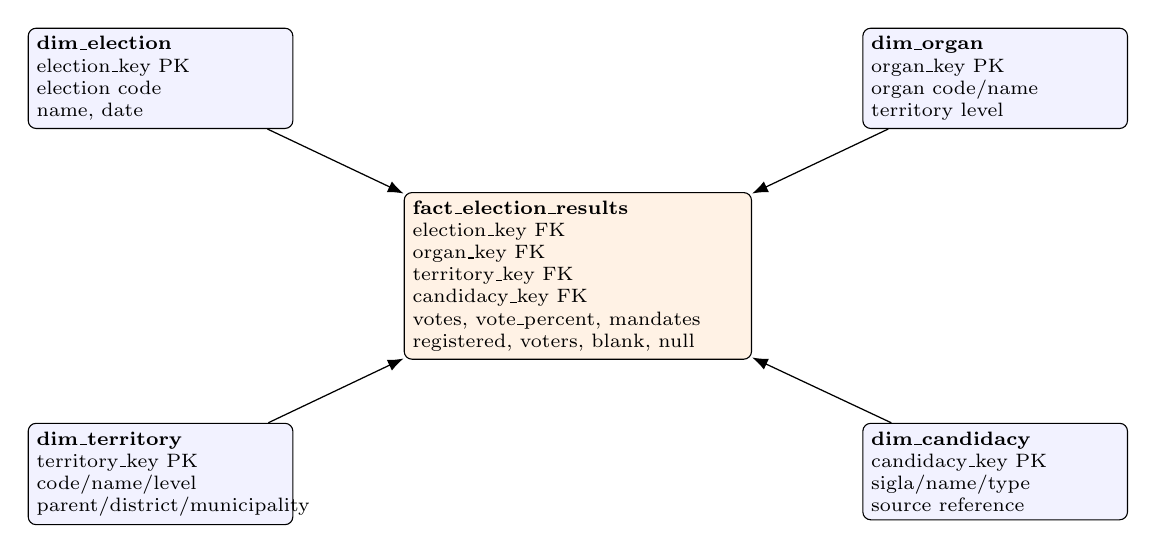
\begin{tikzpicture}[node distance=0.8cm and 1.4cm]
  \node[fact] (fact) {\textbf{fact\_election\_results}\\election\_key FK\\organ\_key FK\\territory\_key FK\\candidacy\_key FK\\votes, vote\_percent, mandates\\registered, voters, blank, null};

  \node[entity, above left=of fact] (de) {\textbf{dim\_election}\\election\_key PK\\election code\\name, date};
  \node[entity, above right=of fact] (do) {\textbf{dim\_organ}\\organ\_key PK\\organ code/name\\territory level};
  \node[entity, below left=of fact] (dt) {\textbf{dim\_territory}\\territory\_key PK\\code/name/level\\parent/district/municipality};
  \node[entity, below right=of fact] (dc) {\textbf{dim\_candidacy}\\candidacy\_key PK\\sigla/name/type\\source reference};

  \draw[rel] (de) -- (fact);
  \draw[rel] (do) -- (fact);
  \draw[rel] (dt) -- (fact);
  \draw[rel] (dc) -- (fact);
\end{tikzpicture}

\caption{Warehouse star schema. The fact table combines vote, mandate, and turnout measures with dimensions for election, organ, territory, and candidacy.}
\label{fig:warehouse}
\end{figure*}

Materialized views are used for frontend performance and repeated analytical access:

\begin{itemize}
  \item \texttt{election.mv\_result\_summary};
  \item \texttt{election.mv\_national\_totals};
  \item \texttt{election.mv\_territory\_winners}.
\end{itemize}

The fact table stores both candidate measures and turnout measures. Although turnout is not candidate-specific, keeping it in the fact table simplifies dashboard queries because each result row can be displayed with the corresponding context. The normalized operational table remains the authoritative source, while the warehouse optimizes analytical access.

The warehouse refresh is destructive and rerunnable: dimensions and facts are truncated and rebuilt from the operational schema. This is acceptable for the project scope because the pipeline loads a fixed official dataset rather than continuously updated production data.

\section{SQL Programming}

The database contains SQL functions, PL/pgSQL procedures, and triggers. The function \texttt{election.vote\_share} computes vote share from votes and valid votes. The function \texttt{election.turnout\_rate} computes turnout. The function \texttt{election.dhondt\_allocate} implements the D'Hondt method using generated divisors and a ranking window function.

The procedure \texttt{election.load\_from\_staging()} transforms staged CNE rows into the operational schema. The procedure \texttt{dw.refresh\_from\_operational()} rebuilds the warehouse and refreshes materialized views.

Triggers enforce consistency:

\begin{itemize}
  \item turnout values cannot be negative, voters cannot exceed registered voters, and blank plus null votes cannot exceed voters;
  \item vote results must match the candidacy scope;
  \item seat results must match the candidacy scope and cannot have negative mandates.
\end{itemize}

The D'Hondt implementation is intentionally implemented in SQL rather than Python. It creates all quotients using \texttt{generate\_series(1, seats)}, ranks them with a window function, and returns the first \texttt{n} quotients. This makes the allocation transparent, testable, and reusable by other SQL queries.

\section{Analytical SQL}

The file \texttt{sql/05\_analytical\_queries.sql} contains examples required by the assignment:

\begin{itemize}
  \item D'Hondt allocation;
  \item three window-function queries;
  \item one \texttt{GROUP BY ROLLUP} query;
  \item one \texttt{GROUP BY CUBE} query;
  \item advanced aggregation using \texttt{FILTER} and \texttt{jsonb\_agg}.
\end{itemize}

The analytical queries support municipality rankings, national vote shares, turnout rankings inside districts, candidate-type subtotals, and district-level winner summaries.

The \texttt{ROLLUP} query produces totals at several levels in one result: candidate totals per district, district totals, and the global total. The \texttt{CUBE} query compares votes and mandates across candidate type and district, including subtotals for both dimensions. These queries demonstrate that the warehouse and operational views support aggregate analysis beyond simple result lookup.

\section{Spatial Data and Frontend}

The \texttt{election.territories} table stores geometries as \texttt{geometry(MultiPolygon, 3763)}. The CAOP loader reads GeoPackage layers for municipalities, districts/regions, and parishes, reprojects them to EPSG:3763, and updates the territory table.

The loaded geometry coverage is:

\begin{table}[h]
\centering
\caption{Loaded CAOP geometry coverage.}
\begin{tabular}{lrr}
\toprule
Level & Total & With geometry\\
\midrule
District/region & 20 & 20\\
Municipality & 308 & 308\\
Parish & 3083 & 2949\\
\bottomrule
\end{tabular}
\end{table}

The assignment minimum is satisfied because all district/region and municipality geometries are loaded. Parish coverage is partial because CAOP 2025 does not match every 2021 parish code exactly, but parish geometry was not required for the minimum scope.

The frontend is a Flask application. It uses explicit SQL through \texttt{psycopg2}; no ORM hides the database logic. The homepage shows a Leaflet municipality map colored by the winning candidacy. The municipality result page shows turnout, a results table, vote-share chart, seat-distribution chart, and elected members when available.

The map endpoint returns a GeoJSON feature collection generated from PostGIS using \texttt{ST\_AsGeoJSON}, \texttt{ST\_Transform}, and \texttt{ST\_SimplifyPreserveTopology}. Geometries are stored in the Portuguese projected CRS for database work and transformed to EPSG:4326 for Leaflet display. Each feature includes municipality code, name, district/region name, winning sigla, vote share, mandates, and turnout.

The frontend has deliberately limited responsibilities. It does not compute election metrics itself; it only sends SQL queries to the database and renders returned values. Charts are produced with Plotly in Python and embedded into the templates. This follows the assignment requirement that the database component remains central.

\section{Validation}

The database was loaded and validated on a local PostgreSQL/PostGIS database named \texttt{tabd}. The main load command was:

\begin{verbatim}
.venv/bin/python etl/load_cne_2021.py \
  --setup --dsn "dbname=tabd"
\end{verbatim}

The validation file \texttt{sql/07\_validation\_queries.sql} checks staging, operational, warehouse, materialized view, and D'Hondt results.

Key validated counts:

\begin{table}[h]
\centering
\caption{PostgreSQL validation counts.}
\begin{tabular}{lr}
\toprule
Table & Rows\\
\midrule
\texttt{staging.cne\_result\_rows} & 3719\\
\texttt{staging.cne\_candidate\_votes} & 12277\\
\texttt{staging.cne\_percent\_mandates} & 12277\\
\texttt{staging.cne\_elected\_members} & 35491\\
\texttt{election.vote\_results} & 12277\\
\texttt{election.seat\_results} & 12277\\
\texttt{dw.fact\_election\_results} & 12277\\
\bottomrule
\end{tabular}
\end{table}

For Agueda's municipal council, the D'Hondt calculation matched the official mandates: PPD/PSD.MPT received 4 mandates, PS received 2, and CDS-PP received 1.

The Flask map endpoint was also tested through the Flask test client. The homepage returned HTTP 200, and the GeoJSON endpoint returned 308 municipality features. The first tested feature was Agueda, with winner PPD/PSD.MPT, 9991 votes, 47.26 percent vote share, 4 mandates, and 52.74 percent turnout. This confirms that the frontend can query both election results and loaded CAOP geometries.

\section{Implementation Files}

The most relevant implementation files are:

\begin{itemize}
  \item \texttt{sql/00\_extensions\_and\_schemas.sql}: schema reset and PostGIS extension;
  \item \texttt{sql/01\_staging\_schema.sql}: CNE staging tables;
  \item \texttt{sql/02\_operational\_schema.sql}: normalized operational schema;
  \item \texttt{sql/03\_warehouse\_schema.sql}: warehouse dimensions and fact table;
  \item \texttt{sql/04\_functions\_views\_triggers.sql}: SQL functions, procedures, triggers, views, and D'Hondt;
  \item \texttt{sql/05\_analytical\_queries.sql}: assignment analytical SQL examples;
  \item \texttt{sql/06\_materialized\_views.sql}: cached frontend/analytics views;
  \item \texttt{sql/07\_validation\_queries.sql}: validation queries;
  \item \texttt{etl/load\_cne\_2021.py}: CNE election ETL;
  \item \texttt{etl/load\_caop.py}: CAOP geometry ETL;
  \item \texttt{app/app.py} and \texttt{app/db.py}: Flask routes and explicit SQL query helpers.
\end{itemize}

\section{Limitations and Extensions}

The main limitation is the use of CAOP 2025 geometries instead of CAOP 2021. This is acceptable as a documented newer compatible official boundary source, but a perfect historical match would use CAOP 2021. Parish geometries are partial because some parish codes changed between 2021 and 2025.

Another limitation concerns elected-member rows: 35491 elected-member rows were parsed, while 35142 were loaded into the operational table. The mismatch comes from parish-level inconsistencies between elected-member labels/codes and normalized candidacies. This does not affect votes, turnout, mandates, D'Hondt, warehouse facts, or municipality-level analysis.

Future extensions include loading additional election years, adding more historical comparisons, improving parish-level reconciliation, adding materialized aggregates for more frontend views, and enriching the frontend with party filters and district comparison pages.

\section{Contributions}

Rui Coelho (up202106772) worked on data inspection, ETL validation, PostgreSQL/PostGIS loading, frontend testing, and documentation.

Ricardo Ribeiro (up202104806) worked on schema design, analytical SQL, D'Hondt validation, report review, and presentation preparation.

AI-assisted programming and documentation support was used during development. The final database design, code, SQL logic, and report contents should be reviewed and understood by both group members before submission.

\section{Reproducibility}

The project can be reproduced by installing dependencies, loading the CNE data, loading CAOP geometries, and running the Flask app:

\begin{verbatim}
python3 -m venv .venv
.venv/bin/pip install -r requirements.txt
.venv/bin/python etl/load_cne_2021.py \
  --setup --dsn "dbname=tabd"
.venv/bin/python etl/load_caop.py \
  --caop-dir . --dsn "dbname=tabd"
.venv/bin/flask --app app/app.py run
\end{verbatim}

\end{document}
